% -----------------------------------------------------------------------------
% November, 2023 update by Eve Torrence
% This file contains a sample Bridges paper in LaTeX format.
% The original was written by Carlo S\'equin in 2017, using previous
% versions by Doug McKenna, Craig Kaplan, Reza Sarhangi, and others,
% with \LaTeX\ contributions by Bruce Torrence and David Swart.
% It has been vetted using TeXShop 5.10 on Mac OS Big Sur (11.6).
% TeXShop is part of the TeX Live distribution, available
% at http://www.tug.org/texlive/
%
% -----------------------------------------------------------------------------

\documentclass[letterpaper,11pt]{article}
\usepackage{amsmath, amsthm, amssymb}    % May not all be necessary
\usepackage{bridges}			% Custom bridges proceedings style
\usepackage{graphicx}			% For including pictures
\usepackage[colorlinks=true, urlcolor=blue, citecolor=black, linkcolor=black]{hyperref}  
							% For formatting (clickable) URLs
\usepackage{subcaption}			% For captioning multi-panel figures

\urlstyle{rm} 					% Display URLs in same font as body text

% -----------------------------------------------------------------------------

\title{Simulating Digital Circuits Using Wang Cubes}

\author{Mathew Kuthur James\textsuperscript{1}
\vspace{10pt}\\
\textsuperscript{1}David Cheriton School of CS, University of Waterloo} % end \author
% superscripts are only needed if there is more than one author

% \date{[Draft as of \today]}	% uncomment to use for your own draft purposes
\date{}					% Suppress any date on submissions

% -----------------------------------------------------------------------------

\begin{document}

\maketitle

% Prevent page number 1 from being printed on the first page.
\thispagestyle{empty}

\begin{abstract}

This document serves as a \LaTeX\ template for the preparation of papers to be
published in the refereed Proceedings of the Bridges Conference. It
contains detailed formatting instructions as well as some general
guidelines for appropriate content of such papers. Adherence to this
template is important, since the Proceedings will be composed directly
from your manuscripts in their final submitted form. Your abstract
should be only one paragraph, comprising anywhere from three to eight
lines of text---the shorter the sweeter. Abstracts will be used
separately from the rest of the paper; please avoid footnotes,
citations, as well as special symbols and formatting.

\end{abstract}

% Bridges papers are usually no more than 8 pages in length.  So
% there's really no need to have numbered sections, unless the
% author really needs to refer to sections by number within the paper's text.  
% So to suppress sequential section numbers, append an asterisk to 
% the \section command, as in:

%%%%%%%%%%%%%%%%%%%%%%%%%%%%%%%%%%%%%%%%%%%
\section*{Some Guide on Content}

% And don't try to mix and match numbered and unnumbered sections; it's one or the other.

Let's start with some advice on the subject matter and content of a
Bridges paper, since this should be an author's first concern. The
Bridges Proceedings are considered a refereed journal, and as such we
are trying to maintain quality standards that will make its papers count
in academic personnel reviews and promotion cases. Thus, most
importantly, every paper should present some novel achievements,
experiments, artwork, and/or insights by the authors. General reviews or
tutorials, cobbled together from various blogs or Wikipedia pages are
not appropriate. Also, keep in mind that the number of pages in the
Proceedings as well as your presentation time at the conference are
limited; so choose a scope for your presentation that fits into these
constraints.

\textbf{Regular papers} should be either 8 or 6 pages, including references. Every paper should nicely
fill an even number of pages without a lot of wasted white space, so
that we can make optimal use of the Proceedings pages and start every
paper on a right-hand page.

\textbf{Short papers}, which have a later submission deadline, should be
4 or 2 pages long, including references. Here it is particularly important to focus 
on just one or two novel ideas and results. Short papers are not a good medium
to give tutorial introductions or cursory reviews over a domain that could be the 
subject of one or more books. Also, this is not the place to give preliminary ideas 
on new teaching experiments, or to present intuitive hunches how some classical 
artwork might be analyzed in a novel way. A Bridges paper should only be submitted 
after the experiments or novel analysis have been performed and when concrete results are available.

The program committee has found that certain types of papers almost always 
need to be rejected: papers on numerology or work that extracts numbers or 
ratios from artwork or architecture. A somewhat ``fuzzy'' search for the Golden 
Ratio (or any other ratio) will almost always produce some hits (a simple matter of 
statistics). However, such coincidences do not tell us anything about the method 
or intent of the creator of those artifacts, unless there is some other
compelling evidence, such as auxiliary lines or notes that explicitly
state what the artist or architect was doing.

Please write your paper in such a way that attendees with a general
education can follow your discourse without the need to look up several
references to find out what the main gist is of your paper. Skip lengthy
sections on \emph{background} and \emph{previous work} and instead give
clear and detailed explanations on your novel contributions, ideally
well-supported with diagrams and/or images.


%%%%%%%%%%%%%%%%%%%%%%%%%%%%%%%%%%%%%%%%%%%
\section*{Use of this Template}

\noindent If you are writing your paper using \LaTeX, please use a
copy of the source \texttt{.tex} file for this document as your starting point. Some 
useful \LaTeX\ resources are \cite{Chang, Gratzer}. This template (with its accompanying 
style file) has been set with the proper paper size and all the necessary \emph{styles} for
proper formatting. Just replace the text in this file with your own text. Also substitute 
your own images for the figures in this template, either as an individual figure like 
Figure \ref{fig:1}, or, alternatively, as in the composite Figure \ref{fig:2}. Each figure is then 
followed by a \verb|\caption|.

\begin{figure}[h!tbp]
	\centering
	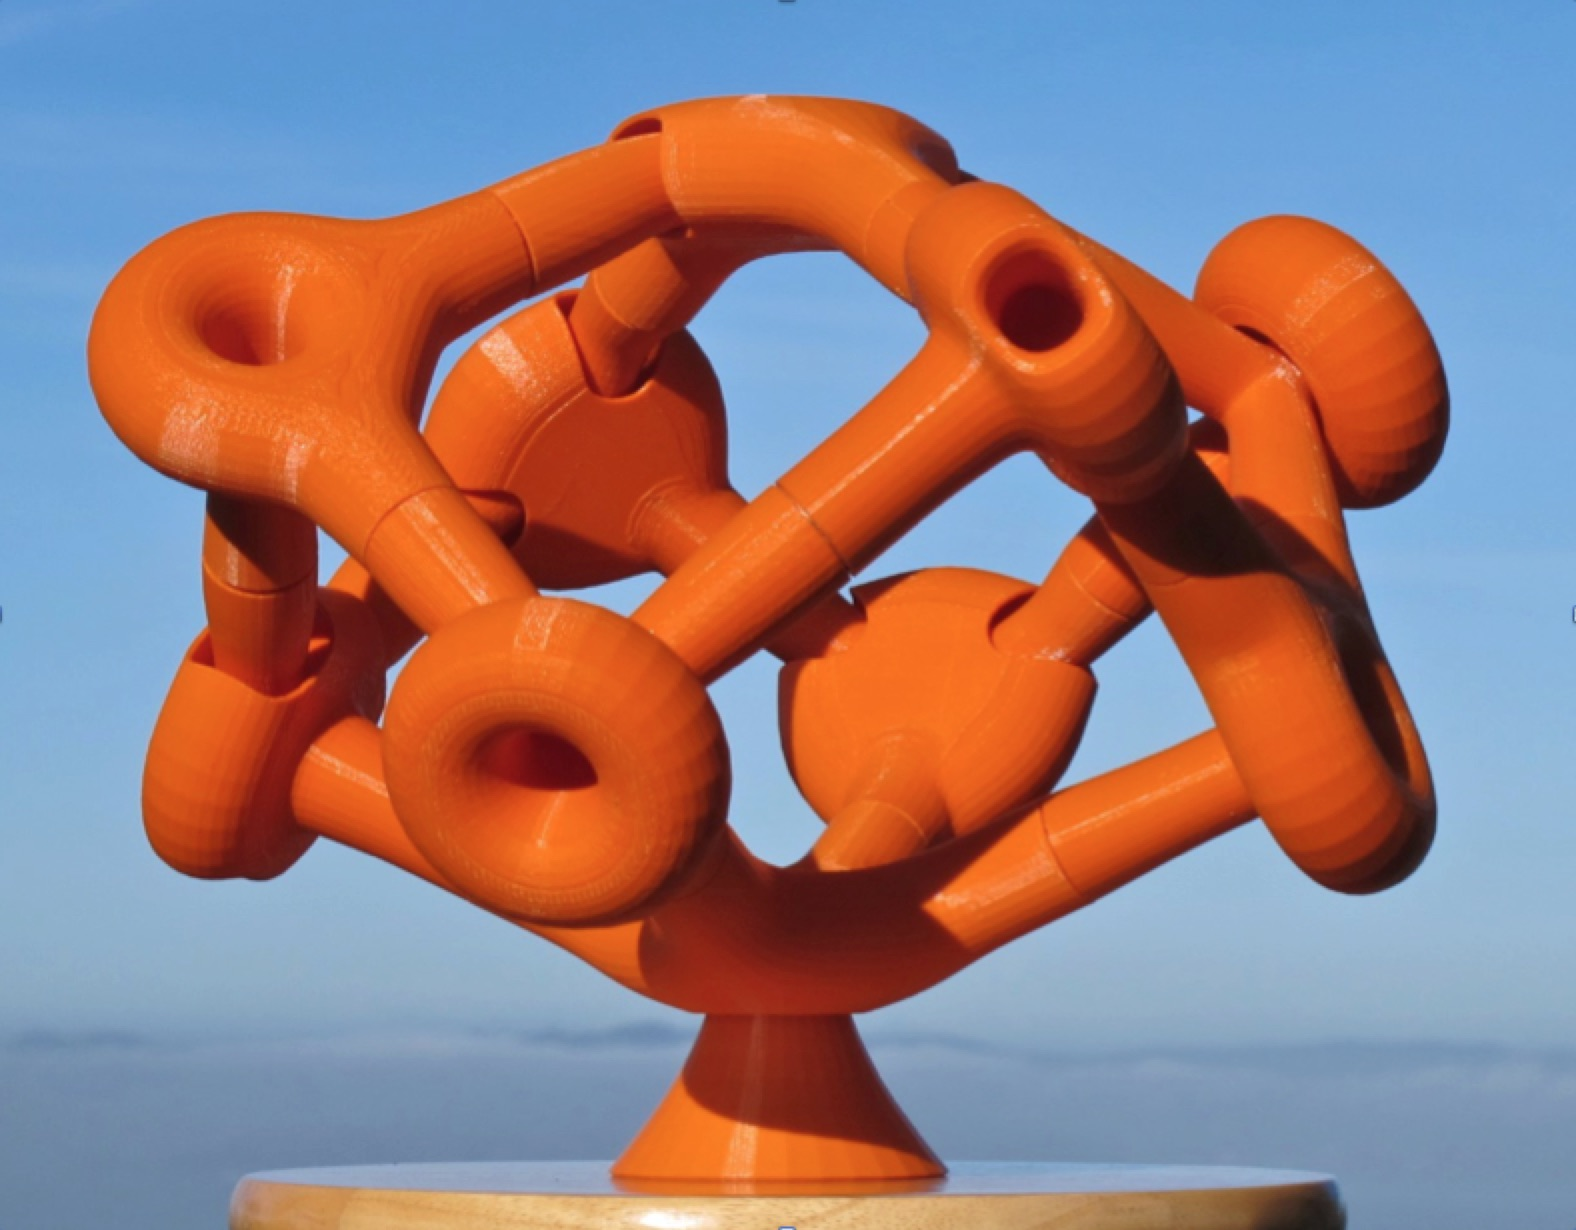
\includegraphics[width=2.4in]{figures/figure1.jpg}
	\caption{An individual figure \cite{Sequin2016}. Make it large enough so that necessary 
	details can be seen.\\ Fine-tune its size, so that you obtain convenient page breaks.}
	\label{fig:1}
\end{figure}



%%%%%%%%%%%%%%%%%%%%%%%%%%%%%%%%%%%%%%%%%%%
\section*{Paper Size, Margins, and Styles}

The Proceedings will be printed using US Letter size paper (8.5 by 11
inches) as in this document. If you are working outside the USA, please
check that you have not used A4 paper, which may be the default in your
country. Do not insert page numbers, headers or footers; these will be
inserted later at the publishing stage.

This template has the proper styles set in the \texttt{bridges.sty} file. 
The result should conform to the following specifications: On the first page, 
the distance from the top edge of the paper to the first line of the title should 
be 3~cm ($1+3/16$ inches). On the second and subsequent pages, the distance 
from the top edge of the paper to the top of the first line of type should be
2.5~cm (1~inch). The widths of the margins on left and right edges and
at the bottom of the page should all be 2.5~cm (1~inch) as well.

The font is \emph{Times New Roman}. The text of the main body,
as well as the figure captions use size 11~pt. Section headings,
authors, and affiliations are size 12~pt. Paper title is 16~pt. Abstract
is 9~pt. Use this template to see what items are printed in \textbf{bold
face} or in \emph{italics}. Use italics for emphasis, rather than blood face (which reads like yelling.)
Mathematical expressions are typeset 
in the same font as the body text, as in $\sqrt{b^2-4ac}$. 

There should be no indentation for the first paragraph after a section heading. Subsequent paragraphs in that section will be indented. The style file will attend to this behavior, and will also justify text to both the left and right margins. 

%%%%%%%%%%%%%%%%%%%%%%%%%%%%%%%%%%%%%%%%%%%
\section*{Figures and Tables}

You must obtain permission and provide attribution to use any copyrighted material. 
Images should be high quality. The proceedings will be produced in full color both online and in print.
But be careful that your images do not make your final PDF larger than 10~Mb;
in that case you may need to downsample your image files to reduce their size.

To insert a figure, use the \emph{figure} environment. For this template, all
image files are placed in the \texttt{images} folder, located in the directory containing the source 
\texttt{.tex} file. Figure captions will be numbered and labeled automatically. Hence the boldface text 
``\textbf{Figure 1:}'' does not need to be typed as part of the figure caption, nor does the 
italic font style need to be specified; these are handled automatically by the Bridges style file.

Figure \ref{fig:2} shows how to format and caption a figure with multiple panels. 
Here we use the \emph{subcaption} package, which enables the \verb|\subcaption| 
command. Leave the subfigure captions blank to automatically label the panels 
(a), (b), etc. We ensure that the full figure does not exceed the width of a full line 
of text by setting the width of each individual panel to be an appropriate proportion of the 
\verb|\textwidth|.

\begin{figure}[h!tbp]
\centering
\begin{minipage}[b]{0.2\textwidth} 
	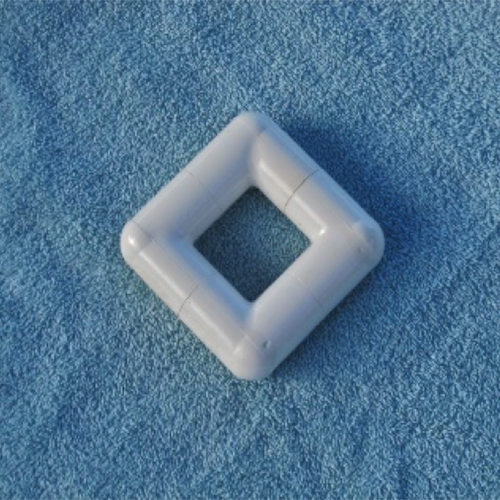
\includegraphics[width=\textwidth]{figures/figure2a.png}
        	\subcaption{} % Add subcaption text if desired, or use \subcaption* to suppress (a), (b), etc. labels
        	\label{fig:2a}
\end{minipage}
~ %add desired spacing between images, e. g., ~, \quad, \qquad, \hfill etc.	
\begin{minipage}[b]{0.2\textwidth} 
	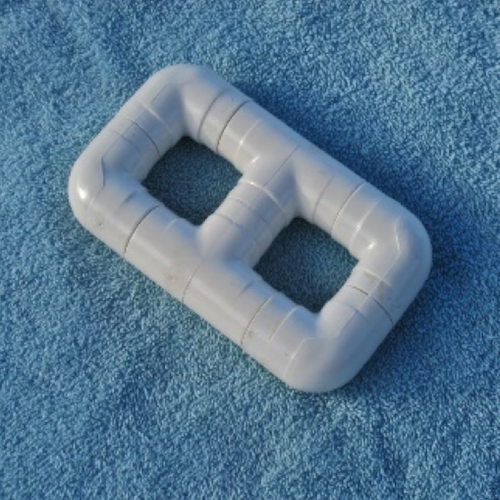
\includegraphics[width=\textwidth]{figures/figure2b.png}
        	\subcaption{} % Add subcaption text if desired, or use \subcaption* to suppress (a), (b), etc. labels
        	\label{fig:2b}
\end{minipage}
~ %add desired spacing between images, e. g., ~, \quad, \qquad, \hfill etc.	
\begin{minipage}[b]{0.2\textwidth} 
	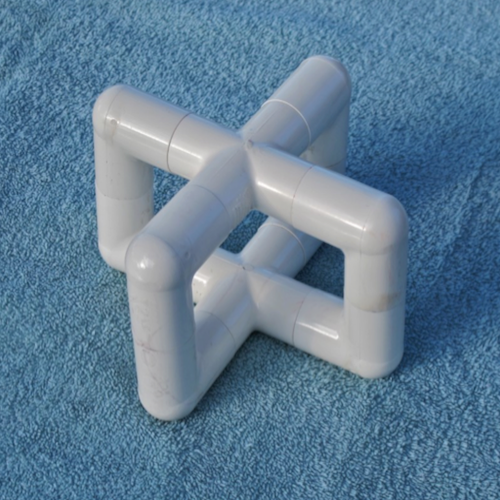
\includegraphics[width=\textwidth]{figures/figure2c.png}
        	\subcaption{} % Add subcaption text if desired, or use \subcaption* to suppress (a), (b), etc. labels
        	\label{fig:2c}
\end{minipage}
~ %add desired spacing between images, e. g., ~, \quad, \qquad, \hfill etc.	
\begin{minipage}[b]{0.2\textwidth} 
	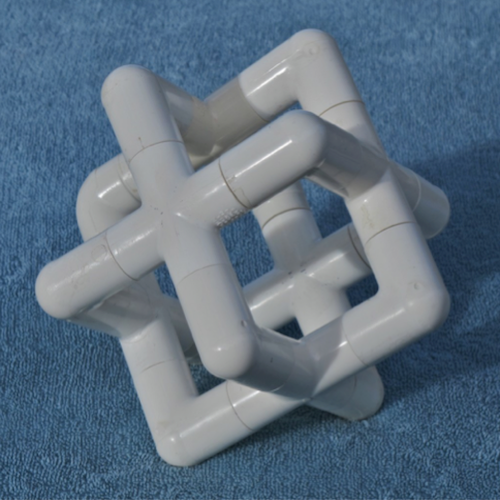
\includegraphics[width=\textwidth]{figures/figure2d.png}
        	\subcaption{} % Add subcaption text if desired, or use \subcaption* to suppress (a), (b), etc. labels
        	\label{fig:2d}
\end{minipage}
\caption{Orientable handle-bodies made from PVC pipe components:  (a) simple torus of genus 1, \\
(b) 2-hole torus of genus 2,  (c) handle-body of genus 3,  (d) handle-body of genus 7.}
\label{fig:2}
\end{figure}
% NOTE: As an alternative, you could use \caption instead of \subcaption for the individual panels, 
% and remove the composite \caption at the bottom. This will produce separate side-by-side figures,
% each with its own Figure number.


Tables are mostly treated just like figures, except that the caption is 
is placed \emph{above} the table body. This is accomplished by placing the 
\verb|\caption| before the table data. In this example we reduce the font size 
in the \emph{tabular} environment so the table fits within the margins. 
All figures and tables must be referenced and explained in the main text, and they must
not bleed into the margins.

\begin{table}[h!tbp]
\centering
\caption{Number of Topologically Different Linkings of Two Cube-Frames.}
{\footnotesize % reduce the font size for entire table
\begin{tabular}{|l|l|l|l|l|l|r|}
\hline
  & 2 edge-loops & 3 edge-loops & 4 edge-loops & 5 edge-loops & 6 edge-loops & total \\
\hline
2 edge-loops & 2sm, 1dm & & & & & 3  \\
\hline
3 edge-loops & 0 & 1sm, 1sp, 2sc, 2dm & & & & 6 \\
\hline
4 edge-loops & 0 & 2dc & 1sm, 10 sc, 2dm, 10dc & & & 25\\  
\hline
5 edge-loops & 0 & 0 & 1dm, 20dc & 16sc, 3dm, 1dp, 24dc & & 65  \\  
\hline
6 edge-loops & 0 & 0 &  3dm, 2dc & 26dc & 14sc & 45\\  
\hline
 & & & & & \multicolumn{1}{r|}{total:} & 144\\
 \hline
 & \multicolumn{2}{c|}{s: swap symmetry} & \multicolumn{2}{c|}{m: mirror symmetry} & & \\
 \hline
 & \multicolumn{2}{c|}{d: different roles for} & \multicolumn{2}{c|}{c: chiral configuration} & \multicolumn{2}{r|}{date: 1/20/2016}   \\
 \hline
 & \multicolumn{2}{c|}{the two frames} & \multicolumn{2}{c|}{p: pseudo chirality} & & \\
 \hline
\end{tabular}
}
\end{table}


%%%%%%%%%%%%%%%%%%%%%%%%%%%%%%%%%%%%%%%%%%%
\section*{Sections and Subsections}

Important words should be capitalized in your paper's title and section
headings, while conjunctions (e.g., ``and'' / ``or'') and prepositions
(e.g., ``of'' / ``with'') begin with a lower case letter. Avoid most punctuation 
(one colon or comma is acceptable). Do not end a lone title or section heading with a period. 
For section headings use \verb|\section*|. Do not use numbered sections
unless you refer to a section by number rather than title in the text. 
If you must have your sections numbered use the \verb|\section| 
command. For any Bridges paper, it would probably be excessive to use 
more than two levels of hierarchy in your document. In all papers the \textbf{Abstract}, 
\textbf{Acknowledgments}, and \textbf{References} headings are unnumbered 
sections.

%%%%%%%%%%%%%
\subsection*{Subsections}

If needed, you may introduce subsections using the command
\verb|\subsection*|. Subsections are never numbered. Subsection titles 
are 11~pt, left justified, bold, and italicized.

%%%%%%%%%%%%%
\subsection*{Vertical Spacing and Page Breaks}

The various styles for headings and paragraphs come with their own
built-in vertical spacing. By default they should result in a good-looking layout. 
But occasionally it is necessary to change vertical spacing a little in order to 
avoid inconvenient page breaks. Try to avoid the last line of a paragraph appearing 
at the beginning of the next page and don't leave a section title on a separate page 
from what follows. Feel free to introduce \verb|\vspace*|
or \verb|\pagebreak| to improve layout.

%%%%%%%%%%%%%
\subsection*{Wrap-up}

% Define BibTeX command for typesetting its logo as it appears the following paragraph -- Feel free 
% to comment this out or delete entirely in your paper.
\def\BibTeX{{\rm B\kern-.05em{\sc i\kern-.025em b}\kern-.08em
    T\kern-.1667em\lower.7ex\hbox{E}\kern-.125emX}}

The paper should end with a brief section that provides some \textbf{Summary and Conclusions}. 
This may be followed by \textbf{Acknowledgments} (optional) and \textbf{References}. Only list 
references that you cite in your paper. List all references alphabetically by last name of first 
author and number them sequentially. When citing references in the text, use \verb|\cite|, as in: 
``see Coxeter \cite{Coxeter}'' or just insert ``\cite{Coxeter}'' after the corresponding quote. 
See the references for correct article \cite{EJCx,Coxeter}, book \cite{Gratzer}, and Bridges 
Conference Proceedings \cite{Sequin2016} citations. Since Bridges papers typically have only 
a few references, we do not require or even recommend that you use \BibTeX, but of course 
you are free to do so. Examples and templates for other types of references can be found in the Guidelines for References section of the Paper Formatting webpage. Don't insert links to references in the body of the paper. 


%%%%%%%%%%%%%%%%%%%%%%%%%%%%%%%%%%%%%%%
\section*{Writing Style and Final Format}

There is no need to use only the passive voice, often encountered in
some formal academic journals. It is perfectly acceptable to use the
first person ``I'' when talking about your own artistic endeavors, and
the inclusive, academic ``we'' works well for more formal statements.

To submit your paper via EasyChair \cite{easychair}, 
you will have to convert it into a PDF (Portable Document Format) file and that file must not exceed 10 MB.
Papers will appear in the online Bridges Archives and in print in full color.



%%%%%%%%%%%%%
\section*{Summary and Conclusions}

Please adhere to the style incorporated in this template, \emph{except} your paper
must end after 2, 4, 6, or 8 pages, \emph{including} references. Substantive
deviations from this style are grounds for rejecting your paper without
any detailed review.


%%%%%%%%%%%%%%%%%%%%%%%%%%%%%%%%%%%%%%%
\section*{Acknowledgements}

Suggestions on how the clarity and usefulness of this guide could be
enhanced would be gladly accepted.

%%%%%%%%%%%%%%%%%%%%%%%%%%%%%%%%%%%%%%%
% References %
    
{\setlength{\baselineskip}{13pt} % tighten line spacing for bibliography
\raggedright				% no right justification for References
\begin{thebibliography}{99}

% \bibitem{Chang}
% W. Chang. \LaTeX\ \textit{Cheat Sheet}. 2014. \url{http://wch.github.io/latexsheet/}.

% \bibitem{EJCx}
% M.\ Chladn\'y and M.\ \v Skoviera. ``Factorisation of Snarks.'' \textit{Electronic Journal
% of Combinatorics}, vol.~17, no.~1, R32, 2010.
% \url{http://www.combinatorics.org/Volume_17/PDF/v17i1r32.pdf}.

% \bibitem{Coxeter} H.\ S.\ M.\ Coxeter. ``The Non-Euclidean Symmetry of Escher's Picture
% Circle Limit III.'' \textit{Leonardo}, vol.~12, no.~1, 1979, pp.~19--25.

% \bibitem{easychair} EasyChair. Log in page. \url{https://easychair.org/account/signin.cgi}.

% \bibitem{Gratzer} G.\ Gr\"atzer. \textit{More Math Into} \LaTeX, 4th ed. Springer, 2007.

% \bibitem{Sequin2016} C.\ H.\ S\'equin. ``From Klein Bottles to Modular Super-Bottles.'' 
% \textit{Bridges Conference Proceedings}, Jyv\"askyl\"a, Finland, Aug. 9--13,
% 2016, pp.~41--48. \url{http://archive.bridgesmathart.org/2016/bridges2016-41.html}.


\bibitem{Merrel} Merrel, Paul. ``Example-based model synthesis'' \textit{Proceedings of the 2007 Symposium on Interactive 3D Graphics and Games}, 2007, pp.105--112 \url{https://doi.org/10.1145/1230100.1230119}



\end{thebibliography}
} % end setlength, raggedright
   
\end{document}